\begin{savequote}[75mm]
Throw two planets into space, and they will fall one on the other...it is a fatality, a question of time; that is all.
\qauthor{Jules Verne}
\end{savequote}

\chapter{An Introduction to the Three-body Problem} \label{s:threebodyproblem}
% \begin{multicols*}{2}
\lettrine{T}{he} three-body problem has admitted a `star-studded line-up' of mathematicians to its' study; names such as \citep{Euler1736}, \citep{Jacobi1829} and \citep{Poincare1899} performed a lot of the early work on its' formulation.

Its' inception is believed to have begun with \citep{Euler1736} [WRONG - 1767], who introduced a synodic coordinate system during his studies of Lunar motion. In fact, this co-ordinate system admitted a constant of motion, later to be `discovered' by \citep{Jacobi1829} to be the well-known Jacobi integral. Euler's work also contained a solution of the motion of a third body under the action of two fixed force centers. Whilst this postulation neglects the centrifugal and Coriolis forces, it yields a solution and thus provides numerous applications. In particular, this solution is sometimes applied as a reference orbit for general-perturbation theory \citep{theoryoforbits}.

One of the next significant contributions came with \citep{Jacobi1829}, who re-discovered -- to the tongue-in-cheek remark of Wintner -- the integral of motion in the three-body problem and his namesake. The Jacobian is an important integral in the three-body problem, for it relates the magnitude of the velocity vector to the location of the third mass. In a system with no solution expressible by algebraic relations, the Jacobi integral can qualitatively imply characteristics of the third body's motion without the solution to the governing equation.

\citep{Hill1906} later used the Jacobi integral to prove that the Earth-Moon distance is bounded from above; the integral predicts a `forbidden region', for which the motion of the third mass cannot enter.

Euler [1772, reference] studied the motion of the Moon assuming the paths of the Earth and the Sun are circular, and that the mass of the Moon was negligible; a study now known as the \textit{restricted three-body problem}. Lagrange [1772, reference] discovered the equilateral triangle solutions; together with the collinear solutions, these solutions are the only explicit solutions for arbitrary masses. 

The classical period of study for the three-body problem ended when the methods of section, phase-space and deterministic chaos were developed by Poincar\'e. For this, Sweden’s King Oscar II awarded Poincar\'e a prize to award him for being the first to solve the n-body problem (although he did not, in fact, even solve the general case of the three-body problem.)

\section{The Newtonian n-body problem}

The following section derives the governing equations of motion for the Newtonian $n$-body problem, as a key piece of background introductory material for the formulation of the three-body problem, a particular case for $n=3$.

We wish to study the motion of a $k$th particle under the influence of $n \geqslant 2$ bodies, which moves in three-dimensional space $x_1, x_2, x_3$ under the influence of Newtonian inverse-square gravitation. We state that the Cartesian coordinates of such a particle are given by $(x_{k1}, x_{k2}, x_{k3}) \in \mathbb{R}^3$ and thus that the differential equations that define the motion of such a particle are given by:

\begin{equation}\label{gravitation}
m_k \ddot{x}_k = \sum_{\substack{j=1 \\ j \neq k}}^{n} \frac{Gm_j m_k}{\pmb{r^2}_{jk}} \frac{\pmb{x}_j - \pmb{x}_k}{r_{jk}}
\end{equation}

for $k = 1, 2, ..., n$ and where $r_{jk} = \lvert \pmb{x}_j - \pmb{x}_k \rvert = \sqrt{\sum_{i=1}^3 (x_{ji} - x_{ki})}$ is the Euclidean distance between the $k$th and $i$th particles. Equation \ref{gravitation} states that the $k$th particle $P_k$ moves under the sum of the forces from the $n-1$ particles $P_n$, $n = 1, 2, 3..., n-1$, and represents $3n$ second-order differential equations.

If we linearise Equation \ref{gravitation} and divide by $m_k$:

\begin{equation}\label{eq:newtonianvelocity}
\begin{aligned}
\dot{\pmb{x}}_k = \pmb{v}_k\\
\pmb{v}_k = m^{-1}_k \frac{\partial U}{\partial \hspace{1pt} \pmb{x}_k}
\end{aligned}
\end{equation}

then we obtain the velocity of the $k$th particle $\pmb{v}_k = (v_{k1}, v_{k2}, v_{k3}) = (\dot{x}_{k1}, \dot{x}_{k2}, \dot{x}_{k3}) \in \mathbb{R}^3$, where $U$ is the potential energy and $G$ the universal gravitational constant.

\begin{equation}\label{eq:newtonianpotentialenergy}
U = \sum_{\substack{j = 1\\ j \neq k}}^n \frac{G m_j}{r_{jk}}
\end{equation}

$\frac{\partial U}{\partial \hspace{1pt} \pmb{x}_k}$ is a real function of three variables that yields $6n$ first order differential equations; further, if $r_{jk} > 0$, then $U$ is smooth -- it has partial derivatives for all orders of variables and is real analytic. Inspection of Equation \ref{eq:newtonianpotentialenergy} reveals that it is of the form $\pmb{\dot{y}} = \textnormal{f}(\pmb{y}); \pmb{y} = (\pmb{x}, \pmb{v}) \in \mathbb{R}^{6n}$, and we can thus apply standard uniqueness and existence theorems (and by implication, also to Equation \ref{eq:newtonianvelocity}). This $(6n + 1)$ dimensional relationship -- $\pmb{x_{kj}}, \pmb{v_{kj}}, t$ -- can be reduced  by finding an integral solution to Equation \ref{gravitation} , which is a real-valued function of the $(6n + 1)$ variables, and is constant through a solution to \ref{gravitation}. If we denote a solution as $\pmb{x}(t), \pmb{v}(t)$, then we arrive at the conclusion that the integral of \ref{gravitation}, $I \hspace{1pt}(\pmb{x, v}, t)$, is such that:

\begin{equation}
\frac{d}{dt} I \onespace (\pmb{x}(t), \pmb{v}(t), t) = 0
\end{equation}

which implies that the integral is constant through the given solution, defining a $6n$-dimensional integral manifold on which the solutions lie.

\begin{equation}
I^{-1}(0) = \lbrace (\pmb{x}, \pmb{v}, t) \in \mathbb{R}^{6n+1} \rvert I = c\rbrace
\end{equation}

This integral constrains the motion of the particle by solving for one variable as a function of the other six. We define the $6n$-dimensional state of coordinates to be the phase space: $(\pmb{x}, \pmb{v}) \in \mathbb{R}^{3n} \times \mathbb{R}^{3n}$ and the extended phase space to be inclusive of the extra dimension $t$: $(\pmb{x}, \pmb{v}, t) = \mathbb{R}^3 \times \mathbb{R}^3 \times \mathbb{R}^1$.

\subsubsection{Algebraic Integrals of the Newtonian $n$-body Problem}

Equation \ref{gravitation} yields 10 independent algebraic integrals, provided by the conservation of momentum -- both linear and angular -- and energy. To begin, we may add \ref{gravitation} to derive linear momentum conservation:

\begin{align}\label{eq:addedgravitation}
\textnormal{LHS:} \sum_{k=1}^n m_k\ddot{\pmb{x}}_k \\
\textnormal{RHS:} \sum_{k=1}^n \sum_{j=1}^n \frac{Gm_j m_k}{r^2_{jk}} \frac{\pmb{x}_j - \pmb{x}_k}{r_{jk}}
\end{align}
The RHS is 0, due to cancellations of negatives from the summation, and thus we may imply:

\begin{equation}\label{eq:zeroCoM}
\sum_{k=1}^n m_k \pmb{\ddot{x}}_k = 0
\end{equation}

\noindent If we take the vector centre of mass for the particles to be $\pmb{\rho} = (\rho_1, \rho_2, \rho_3) \in \mathbb{R}^3$, and thus $\pmb{\ddot{\rho}} = 0$:

\begin{equation}
M = \sum^n_{k=1} m_k, \hspace{5pt} \rho = M^{-1} \sum^n_{k=1} m_k \pmb{x}_k
\end{equation}

\noindent Yielding:

\begin{equation}\label{eq:newtonianlinearmomentum}
\pmb{\rho} = \pmb{c_1}t + \pmb{c_2}
\end{equation}

\noindent where $\pmb{c_1}, \pmb{c_2}$ provide six constants to be unique from the initial conditions at $t = t_0$ \footnote{Note that Equation \ref{eq:newtonianlinearmomentum} gives the law of the conservation of linear momentum -- that the center of mass moves uniformly in a straight line.}.

For analysis, we may move the origin of the Cartesian coordinate system $x_1, x_2, x_3$ for motion of the $k$th particle through a shift:

\begin{equation}
\bar{x}_j = x_j - \rho_j
\end{equation}

\noindent without alteration of Equation \ref{gravitation}, since $\ddot{\rho}_j = 0$. An assumption can therefore be made that $\pmb{\rho} = 0$, and as such:

\begin{equation}
\sum^n_{k=1} m_k \pmb{x}_k = 0, \hspace{5pt} \sum^n_{k=1} m_k \pmb{v}_k
\end{equation}

\noindent which represent six independent algebraic integrals. Considering the conservation of energy:

\begin{equation}
\xi = \textnormal{KE} - \textnormal{U}
\end{equation}

\noindent where $U$ is the potential energy, as before, and KE the kinetic energy of the system:

\begin{equation}
\textnormal{KE} = \frac{1}{2} \sum^n_{k=1} m_k \lvert \pmb{v}_k \rvert ^2
\end{equation}

\noindent and is thus our 7\textsuperscript{th} integral, since Equation \ref{eq:newtonianpotentialenergy} implies that the time derivative of $T - U = 0$\footnote{Energy is constant along solutions.}.

The 8\textsuperscript{th}, 9\textsuperscript{th} and 10\textsuperscript{th} integrals are provided by the conservation of angular momentum, using the vector cross product of Equation \ref{gravitation} $\pmb{x}_k \times \pmb{\ddot{x}}_k$:

\begin{equation}\label{eq:newtonianangular}
\sum_{k=1}^n m_k (\pmb{x}_k \times \pmb{\ddot{x}}_k = \sum_{k=1}^n \sum_{j=1}^n \frac{G m_j m_k}{r^3_{jk}} \pmb{x}_k \times \pmb{x}_j = 0
\end{equation}

\noindent $j \neq k$ since $\pmb{x}_k \times \pmb{x}_k = 0$ and $\pmb{x}_k \times \pmb{x}_j = -\pmb{x}_j \times \pmb{x}_k$. Integrating the LHS of \ref{eq:newtonianlinearmomentum} reports:

\begin{equation}\label{eq:newtonianangularcons}
\sum_{k=1}^n \pmb{x}_k \times \pmb{v}_k = \pmb{c}
\end{equation}
$\pmb{c} = (c_1, c_2, c_3) \in \mathbb{R}^3$\footnote{For more information regarding the implication of the value of this constant on the state of the system, refer to \citep{Belbruno2004}}.

\section{The Circular-Restricted Three-Body Problem}

The establishment of some sort of geometric model is necessary for the computation of the secondary mass $m_3$. We define an intertially-fixed coordiate system with its' origin at the barycenter of the primary masses \citep{Mains1993} in the $\bar x,~\bar y,~\bar z$ axes. The $\bar x$ and $\bar y$ axes are in the plane of the two primaries, with $\bar z$ completing the right-handed coordinate system. 

Another system, the rotating coordiante system, is also located at the barycenter of the system, with its' $\bar X$ axis directed from the larger primary to the smaller primary. The $\bar Z$ axis is coincident with its' partner $\bar z$ axis, with $\bar Y$ completing the coordinate system. We define $\theta$ as the angle between the respective $\bar x$ and $\bar X$ coordinate systems. The angular velocity of the system is constant.


\begin{Figure}
\centering
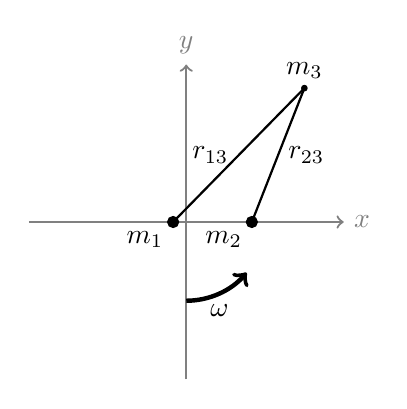
\begin{tikzpicture}

\draw[gray, thick, ->] (-2, 0) -- (2, 0) node[anchor=west] {$x$};		% x-axis
\draw[gray, thick, ->] (0, -2) -- (0, 2) node[anchor=south] {$y$};		% y-axis
\filldraw[black] (-.167, 0) circle (2pt) node[anchor=north east] {$m_1$};
\filldraw[black] (1-.167, 0) circle (2pt) node[anchor=north east] {$m_2$};
\filldraw[black] (1.5, 1.7) circle(1pt) node[anchor=south] {$m_3$};
\draw[black, thick] (-.167, 0) -- (1.5, 1.7) node[anchor=east, midway] {$\pmb{r}_{13}$}; 
\draw[black, thick] (1-.167, 0) -- (1.5, 1.7) node[anchor=west, midway] {$\pmb{r}_{23}$};
\draw[black, ->, ultra thick] (0, -1) arc (270:320:1) node[anchor=north, midway] {$\omega$};

\end{tikzpicture}
\captionof{figure}{Rotating co-ordinate system used in the formulation of the governing equations of motion in the three-body problem.}
\label{f:coordinatesystem}
\end{Figure}

We wish now to use this general form for $n$-body motion to determine the motion of a mass $m_3$ under the influence of two far larger masses $m_1$ and $m_2$, $m_1 > m_2$. Returning to Equation \ref{gravitation} and setting the number of particles $n=3$:

\begin{equation}\label{eq:newtonian3}
\sum F = \frac{Gm_3m_2}{r^3_{23}}\pmb{r_{23}} - \frac{Gm_3m_1}{r^3_{13}} \pmb{r_{13}} = m_3 \ddot{\pmb{r}_3}
\end{equation}

\noindent we may use a number of assumptions to simplify our analysis. Namely:

\begin{itemize}
\item We assume that, for generality, $m_1 > m_2 >> m_3$;
\item Orbits are circular and occur about the pmbycenter of the system;
\item Only gravitational forces act on the masses;
\item The masses are of a sufficient size and characteristic to regard them as point masses.
\end{itemize}


\begin{table*}[t]\label{tbl:normalisations}
\centering
\begin{tabular}{l r}
\toprule
\toprule
Mass parameter & $\mu = \frac{m_2}{M}$ \\
Mass of $m_2$ & $\mu$\\
Mass of $m_1$ & $1 - \mu$\\
Coordinates of the center of mass of $m_1$ & $\rho_1 = (-\mu, 0)$\\
Coordinates of the center of mass of $m_2$ & $\rho_2 = (1-\mu, 0)$\\
Gravitational constant $G$ &  $1$\\
Angular velocity of the system & $1$\\
Period of the two larger masses & $2\pi$\\
\bottomrule
\bottomrule
\end{tabular}
\caption{Normalisations used in the CR3BP}
\end{table*}

\noindent Further, we normalise the system using the mass parameter $\mu$, defined as in Equation \ref{eq:massparameter}:

\begin{equation}\label{eq:massparameter}
\mu = \frac{m_2}{M}, \hspace{3pt} M = m_1 + m_2
\end{equation}

\noindent which implies the normalisations outlined in Table \ref{tbl:normalisations}. If we non-dimensionalise Equation \ref{eq:newtonian3}, we obtain Equation \ref{eq:nondimnewtonian3}.

\begin{equation}\label{eq:nondimnewtonian3}
\ddot{\pmb{r}}^i_{m_3} = -\frac{1-\mu}{r^3_{13}}\pmb{r}_{13} - \frac{\mu}{r^3_{23}} \pmb{r}_{23}
\end{equation}

\noindent Considering the inertial frame of reference, we express the velocity of $m_3$ using the rotating frame and the angular velocity:

\begin{equation}
\dot{\pmb{r}}^I_{m_3} = \pmb{r}^R_{m_3} + \omega_{I\times R} \times \pmb{r}_{m_3}
\end{equation}

\noindent recalling that $\omega_{I\times R}$ is unity, and thus $\omega_{I\times R} = \hat{\gamma} = \hat{z}$ we may write in the inertial frame:

\begin{equation}
\dot{\pmb{r}}_{m_3} = (\dot{x} - y)\hat{x} + (x+\dot{y})\hat{y} + \omega_{I\times R} \times \pmb{r}_{m_3} = (\dot{x} - y)\hat{x} + (x+\dot{y})\hat{y} + \dot{z}\hat{z}
\end{equation}

\noindent and the derivative with respect to time yields Equation \ref{eq:timederivative}.

\begin{equation}\label{eq:timederivative}
\ddot{\pmb{r}}^i_{m_3} = (\ddot{x} - 2\dot{y} - x)\hat{x} + (\ddot{y} + 2\dot{x} - y)\hat{y} + \ddot{z}\hat{z}
\end{equation}

\noindent Equating Equations \ref{eq:nondimnewtonian3} and \ref{eq:timederivative} gives the following:

\begin{equation}\label{eq:governingequations}
(\ddot{x} - 2\dot{y} - x)\hat{x} + (\ddot{y} + 2\dot{x} - y)\hat{y} + \ddot{z}\hat{z} = -\frac{1-\mu}{r^3_{13}}\pmb{r}_{13} - \frac{\mu}{r^3_{23}} \pmb{r}_{23}
\end{equation}

\noindent and we thus arrive at the system of equations that governs the motion of the mass $m_3$, with $r^2_{13}$ and $r^2_{23}$ the Eucliean distances between the primary and secondary to the third body, respectively:

\begin{align}\label{eq:euclideandistances}
r^2_{13} = (x+\mu)^2 + y^2 + z^2 \\
r^2_{23} = (x - 1 + \mu)^2 + y^2 + z^2
\end{align}

As mentioned previously, the three-body problem admits an integral of motion, the Jacobi constant. To determine this, we first seek to formulate a pseudo-potential, $\Omega$, through integrations of the right-hand side of Equation \ref{eq:governingequations}, with respect to the variables $x, y$ and $z$, respectively:

\begin{align}
\Omega_x = \frac{x^2}{2} + \frac{1 - \mu}{r_13} + \frac{\mu}{r_{23}} + f(y, z) \\
\Omega_y = \frac{y^2}{2} + \frac{1 - \mu}{r_{13}} + \frac{\mu}{r_{23}} + f(x, z) \\
\Omega_z = \frac{1 - \mu}{r_1} + \frac{\mu}{r_{23}} + f(x, y)
\end{align}

\noindent Which we may write as a function of particle position and the mass parameter only.

\begin{equation}\label{eq:pseudopotential}
\Omega = \frac{1}{2} (x^2 + y^2) + \frac{1 - \mu}{r_{12}} + \frac{\mu}{r_{23}}
\end{equation}

\noindent As a result, with slight rearranging, we may report the governing equations of motion in Equation \ref{eq:governingequations} as functions of the pseudo-potential.

\begin{align}\label{eq:governingequationspseudopotential}
\ddot{x} - 2\dot{y} = \frac{\partial \Omega}{\partial x} \\
\ddot{y} + 2\dot{x} = \frac{\partial \Omega}{\partial y} \\
\ddot{z} = \frac{\partial \Omega}{\partial z} 
\end{align}


% \begin{figure*}[ht]
% \centering
% \begin{subfigure}{.45\textwidth}
% \centering
% \includegraphics[width=\linewidth]{figures/potential90}
% \end{subfigure}%
% \begin{subfigure}{.45\textwidth}
% \centering
% \includegraphics[width=\linewidth]{figures/potential30}
% \end{subfigure}
% \caption{Plots of the Pseudo-potential in the Earth-Moon system; $\mu = 6$.}
% \label{f:pseudopotential}
% \end{figure*}


% \begin{Figure}
% \centering
% \includegraphics[width=.8\linewidth]{figures/potential90}
% \captionof{figure}{Plots of the Pseudo-potential in the Earth-Moon system; $\mu = 6$.}
% \label{f:pseudopotential}
% \end{Figure}

Figure \ref{f:pseudopotential} reports a plot of the pseudo-potential in the Earth-Moon system; the measurement of the position and velocity of the mass $m_3$ determines the energy associated with its' motion.

\begin{figure}
\centering
\includegraphics[height=.3\textheight]{figures/pseudoPotential}
\captionof{figure}{The pseudo-potential in the Earth-Moon system for $\mu$ = 6}
\label{f:pseudopotential}
\end{figure}


\subsubsection{The Jacobi Constant}

The Jacobi integral admits the constant of motion for the three-body problem. We may derive the Jacobi integral from the equations of motion in \ref{eq:governingequations}:

\begin{equation}
\frac{\textnormal{d}}{\textnormal{d}t} ( \dot{x}^2 + \dot{y}^2 + \dot{z}^2 ) = 2(\dot{x}\ddot{x} + \dot{y}\ddot{y} + \dot{z}\ddot{z})
\end{equation}

\noindent which, when including expressions for $\ddot{x}$ and the other position variables from Equation \ref{eq:governingequationspseudopotential}, reads:

\begin{flalign}
\frac{\textnormal{d}}{\textnormal{d}t} ( \dot{x}^2 + \dot{y}^2 + \dot{z}^2 ) \\ = 2[\dot{x}(2\dot{y} - \Omega_x) + \dot{y}(-2\dot{x} - \Omega_y) + \dot{z}(-\Omega_z)] = 2\frac{\textnormal{d}}{\textnormal{d}t} (-\Omega)
\end{flalign}

\noindent and thus, we obtain the Jacobi constant:

\begin{equation}\label{eq:jacobiconstant}
C = - (V^2 + \Omega), \hspace{2pt} V = (\dot{x}^2 + \dot{y}^2 + \dot{z}^2)
\end{equation}

\noindent which represents the energy state of the mass $m_3$. 

\section{Forbidden Regions}

With the determination of the value of the Jacobi constant in Equation \ref{eq:jacobiconstant}, we may inspect the concept of forbidden regions, or Hill's curves, from the namesake \citep{Hill1906}. Noting that the energy state is dependent on the velocity and position of the particle only, a given value of the energy integral will permit motions in only certain regions of the three-body system. For example, consider the cases outlined in Figure \ref{f:jacobiconstants}:


\begin{figure*}
\centering
\includegraphics[height=.45\textheight]{figures/jacobiConstantEMSys}
\caption{Forbidden regions in the Earth-Moon system for different values of the Jacobi constant; the forbidden regions are shaded in grey; the value of $C = 3.92$, where the inner and outer regions have just become available to the particle, are of the most interest.}
\label{f:jacobiconstants}
\end{figure*}



\begin{itemize}
	\item $C = 5.00$: here, the energy of the mass $m_3$ is relatively small (for example, consider a spacecraft after injection into LEO), and the regions of travel for the spacecraft are similarly limited. The spacecraft possesses the energy necessary to move along any path that is perturbation free within the vicinity of the larger mass $m_1$ -- this is often named the `interior realm'
	\item Suppose the spacecraft makes a maneouvre to increase its' velocity -- and thus energy -- to a value $C = 4.2$. This opens up a new region of space available for exploration along a perturbation-free path with the `necking' of the Earth-Moon line.
	\item For increasing values of C, for example $C = 3.92$, more regions of space becomes available for the mass to access, leading to the access to the `exterior realm'. Eventually, as is with the case $C = 3.2$, the entire Earth-Moon system is available for traversal (although such a scenario is unfavourable for many locations: we seek to arrive at a point with the least amount of energy expended.)
\end{itemize}


The motion for which we are most interested in is for case 3, when the spacecraft may traverse either the exterior or interior regions through means of motion through the `neck' point around the second primary. We will discover in Section \ref{s:manifoldstuff} that the motion in this region is controlled by the invariant manifold structures in the region.

\section{Simplified Motion around the Lagrangian Points}\label{s:lagriangianmotion}

We focus particularly on case 3, where the movement between the exterior and interior realm is controlled by motion through the `neck' region. In this section, we examine the motion of a particle around the lagrangian points as a precursor for trajectories in the neck region, and examine linearisations and characteristics of the motion around these points.

We begin by considering the Lagriangian case of motion expressed in Equation \ref{eq:governingequationspseudopotential}, and translating the origin of the frame to one of the collinear points $L_i$. Denoting $\phi$ to be the distance from $L_i$ to the smaller primary (positive when referring to $L_2$ and negative with respect to $L_1$ and $L_3$), we obtain the new positional coordinates $x^\prime$, $y^\prime$ and $z^\prime$:

\begin{align}
x^\prime = x - (1-\mu + \phi) \\
y^\prime = y\\
z^\prime = z
\end{align}

and for which the linearisation of Equation \ref{eq:governingequations} under this transformation yields:

\begin{align}
\ddot{x}^\prime - 2\dot{y}^\prime - (1+2\alpha)x^\prime = 0 \\
\ddot{y}^\prime + 2\dot{x}^\prime + (\alpha - 1)y^\prime = 0\\
\ddot{z}^\prime + \alpha z^\prime = 0
\end{align}

where $\alpha$ is a constant coefficient. Whilst the solution for the $z$-plane motion is simple harmonic, the in-plane $x-y$ motion involves a characteristic equation in real and imaginary domains; each root represents a mode of motion, one divergent and one non-divergent ADD IN LOW-ENERGY LUNAR REFERENCE HERE. Exciting the non-divergent mode of motion represents a bounded solution.

\begin{align}\label{eq:amplitudeeequations}
x\Prime = -kA_y \cos{(\lambda t + \psi)}\\
y\Prime = A_y\sin{(\lambda t + \psi)}\\
z\Prime = A_z\sin{(\sigma t + \beta)}\label{eq:amplitudeequationsIII}
\end{align}

Equations \ref{eq:amplitudeeequations} through \ref{eq:amplitudeequationsIII} represent six variables in the mode of motion; $A_y$ and $A_z$ represent the amplitudes of in-plane and out-of-plane motion, respectively; $\lambda$ and $\sigma$ the frequency of oscillations in the in- and out-of-planes, and the phase angles for the two planes, $\psi$ and $\beta$. Indeed, it simple to conclude that the solutions to motion around the Lagrange points are characterised by oscillatory motion. With respect to the two frequencies $\lambda$ and $\sigma$, two distinct cases of orbit types emerge:

\begin{itemize}
\item If the two frequencies are commensurate \footnote{From \citep{euclid}: two linked variables are commensurate if their ratio is a rational number.}, the resulting motion is periodic; further, if these are equal, the particle will enter into a halo orbit.
\item If the two frequencies are incommensurate, the motion is quasiperiodic, commonly known as Lissajous  orbits.
\end{itemize}

Further, setting $A_z$ to zero and thus constraining the motion into the $x-y$ plane will yield Lyapunov orbits. Lyapunov orbits have dynamics well represented by the relatively simple linearised dynamics provided above, and may thus be formulated analytically.

Figure \ref{f:lyapunov} provides an example of sets of Lyapunov orbits; note that the three-body problem exhibits symmetry about $y=0$. As a result, there are two families of each type of orbit: `northern' and `southern' orbits. Particles are categorised into each depending on the dominant amount of time spent in each region.

We will see in Section \ref{s:haloorbits} a more advanced method of constructing Halo orbits using forward shooting and differential correction.

% \end{multicols*}
